% 19.11.2025; 13:11:53


\section{Einführung Coding-Paradigmen}%
\begin{frame}%
    \frametitle{Paradigmen -- Einführung}

    \begin{outline}
        \0 \large Unterteilung:
            \1 \textbf{Imperative}-Programmierung
                \2 \textbf{Objekt-Orientierte}-Programmierung (OOP)
                \vspace{.3em}
            \1 \textbf{Deklarative}-Programmierung
            \vspace{3em}
            \0 Unterscheidung: \textbf{State-Frage}!
    \end{outline}

\end{frame}




\note {
    \begin{outline}
        \0 \large Unterteilung:
            \1 \textbf{Imperative}-Programmierung (Kennt ihr schon)
                \2 \textbf{Objekt-Orientierte}-Programmierung (OOP) (Kennt ihr auch schon)
            \1 \textbf{Deklarative}-Programmierung
            \0 Unterscheidung: \textbf{State-Frage!}
    \end{outline}
}



\begin{frame}%
    \frametitle{Paradigmen -- State-Frage}

    \begin{outline}
        \0 Was ist State?
            \1 Anwendungszustand
            \1 Die Gesamtheit des Zustands in dem sich ein Programm befindet
            \vspace{.3em}
        \0 State Frage: Wie wird \textbf{state} in einer Anwendung gehandhabt?
    \end{outline}

\end{frame}
\note {
    \begin{outline}
        \0 Was ist State?
            \1 Anwendungszustand
            \1 Die Gesamtheit des Zustands in dem sich ein Programm befindet
            \vspace{.3em}
        \0 State Frage: Wie wird \textbf{state} in einer Anwendung gehandhabt?
    \end{outline}
}


\subsection{Imperative Programmierung}%
\label{sub:Imperative Programmierung}

\begin{frame}[fragile]
    \frametitle{Paradigmen -- Imperative Programmierung}

    \vfill
    \begin{minipage} {.4\linewidth}\vspace{.3em}%
    \begin{minted}[linenos=false]{python}
werte = [1,2,3,4,5]
summe = 0
for wert in werte:
    summe = summe + wert
\end{minted}
\end{minipage}
\hspace{5em}
\begin{minipage}{.4\linewidth}
    \begin{figure}[H]
        \centering
        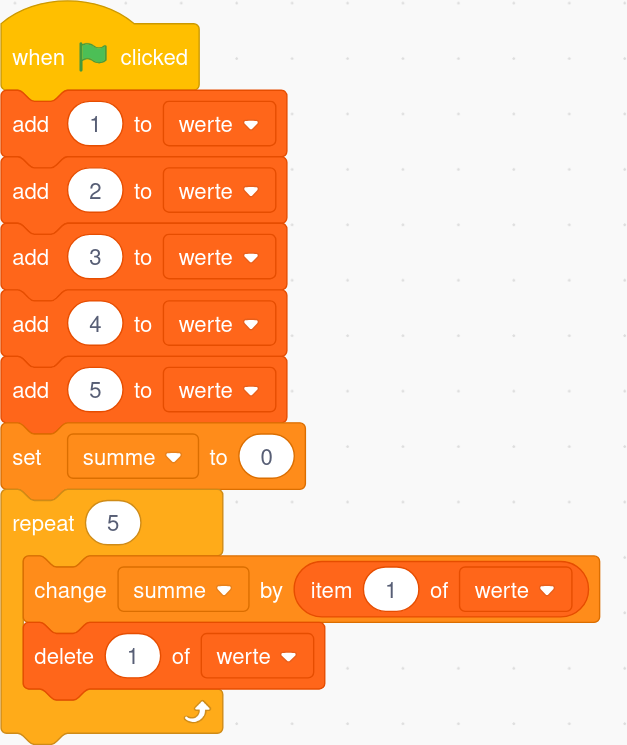
\includegraphics[width=\linewidth]{assets/2025-11-19-14-36-19.png}
    \end{figure}

\end{minipage}
\end{frame}
\note{
    \begin{outline}
        \1 Beispiel
        \1 Auch gutes Beispiel für die Mächtigkeit von Python vs Scratch
    \end{outline}
}

\begin{frame}[fragile]%
    \frametitle{Paradigmen -- Imperative Programmierung}

    \begin{outline}
        \0 Imperative Programmierung
            \1 Anwendungszustand muss bei jeder Anweisung berücksichtigt werden
            \1 Beschreibt wird \textbf{wie} etwas durchgeführt wird
    \end{outline}


\end{frame}

\note {
    \begin{outline}
        \1 Kennt ihr schon
        \1 Reguläre Programmierung, alles was für euch halbwegs intuitiv ist
        \1 Keine Klassen
        \1 Untertypen
            \2 z.b. methodische Programmierung (funktionen)

        \1 Anwendungszustand muss bei jeder Anweisung berücksichtigt werden
            \2 state ist extern zum code
        \1 Beschreibt wird \textbf{wie} etwas durchgeführt wird
            \2 Wir geben den Computer eine Anleitung
            \2 klingt so als gäbe es keine alternative, gibt es aber
    \end{outline}
}


\subsection{Objekt-Orientierte-Programmierung}%
\begin{frame}[fragile]%
    \frametitle{Paradigmen -- Objekt-Orientierte Programmierung}


    \begin{minipage} {\linewidth}\vspace{.3em}%
    \begin{minted}[linenos=false]{python}
class Person
    def __init__(self, name):
        self.name = name
    def greet(self):
        print(self.name + " says hello!")

ada = Person("Ada Lovelace")
ada.greet()

alan = Person("Alan Turing")
alan.greet()
\end{minted}
\end{minipage}

\end{frame}

\note {
    \begin{outline}
        \1 Bsp
    \end{outline}
}
\begin{frame}
    \frametitle{Paradigmen -- Objekt-Orientierte Programmierung}
    \begin{outline}
        \0 Objekt-Orientierte Programmierung
            \1 Anwendungszustand wird in Klassen gekapselt (Datenkapselung)
            \2 Kein globaler\footnote{global = von überall sichtbar/veränderbar} State; State ist lokal\footnote{lokal = nur lokal sichtbar/veränderbar}
                \vspace{.3em}
            \1 Beschreibt wird \textbf{wie} etwas durchgeführt wird
        
    \end{outline}
    
\end{frame}
\note {
    \begin{outline}
        \0 Objekt-Orientierte Programmierung
            \1 Anwendungszustand wird in Klassen gekapselt (Datenkapselung)
                \2 Kein globaler State!
                \2 d.h. State sollte nicht unnötig außerhalb derselben Klasse verfügbar sein.
                    \3 Globaler state: Überall sichtbar/veränderbar
                    \3 lokaler state: Nur lokal (z.B. in der selben Klasse) sichtbar
            \1 Beschreibt wird \textbf{wie} etwas durchgeführt wird
            
    \end{outline}
}


\subsection{Deklarative Programmierung}%
\begin{frame}[fragile]
    \frametitle{Paradigmen Deklarative Programmierung}
    \begin{outline}
        \0 Deklarative Programmierung\\
        \vspace{1.4em}
        \0 \textbf{Zielsetzung:}
        \vfill
            \1 (Veränderlicher) Anwendungszustand existiert nicht.
                \2 Setzen wir einmal eine variable dürfen wir sie nicht verändern
                \2 State wird in Funktionen ""gekapselt"", state darf nicht außerhalb von Funktionen erscheinen
                \vfill

            \begin{minipage} {.3\linewidth}
\begin{minted}[escapeinside=||] {python}
|\sout{\texttt{a = 100}}|
def main():
    a = 1
    b = 2
    print(a+b)
\end{minted}
            \end{minipage}
            \begin{minipage} {.3\linewidth}
\begin{minted}[escapeinside=||] {python}
def main():
    a = 1
    b = 2
    |\sout{\texttt{c = a + b}}|
    print(c)

\end{minted}
            \end{minipage}
            \begin{minipage} {.3\linewidth}
\begin{minted}[escapeinside=||] {python}
def add(a,b):
    return a + b

def main():
    a = 1
    b = 2
    print(add(a,b))
\end{minted}
        \end{minipage}
\end{outline}
\end{frame}

\note {
~\\{\centering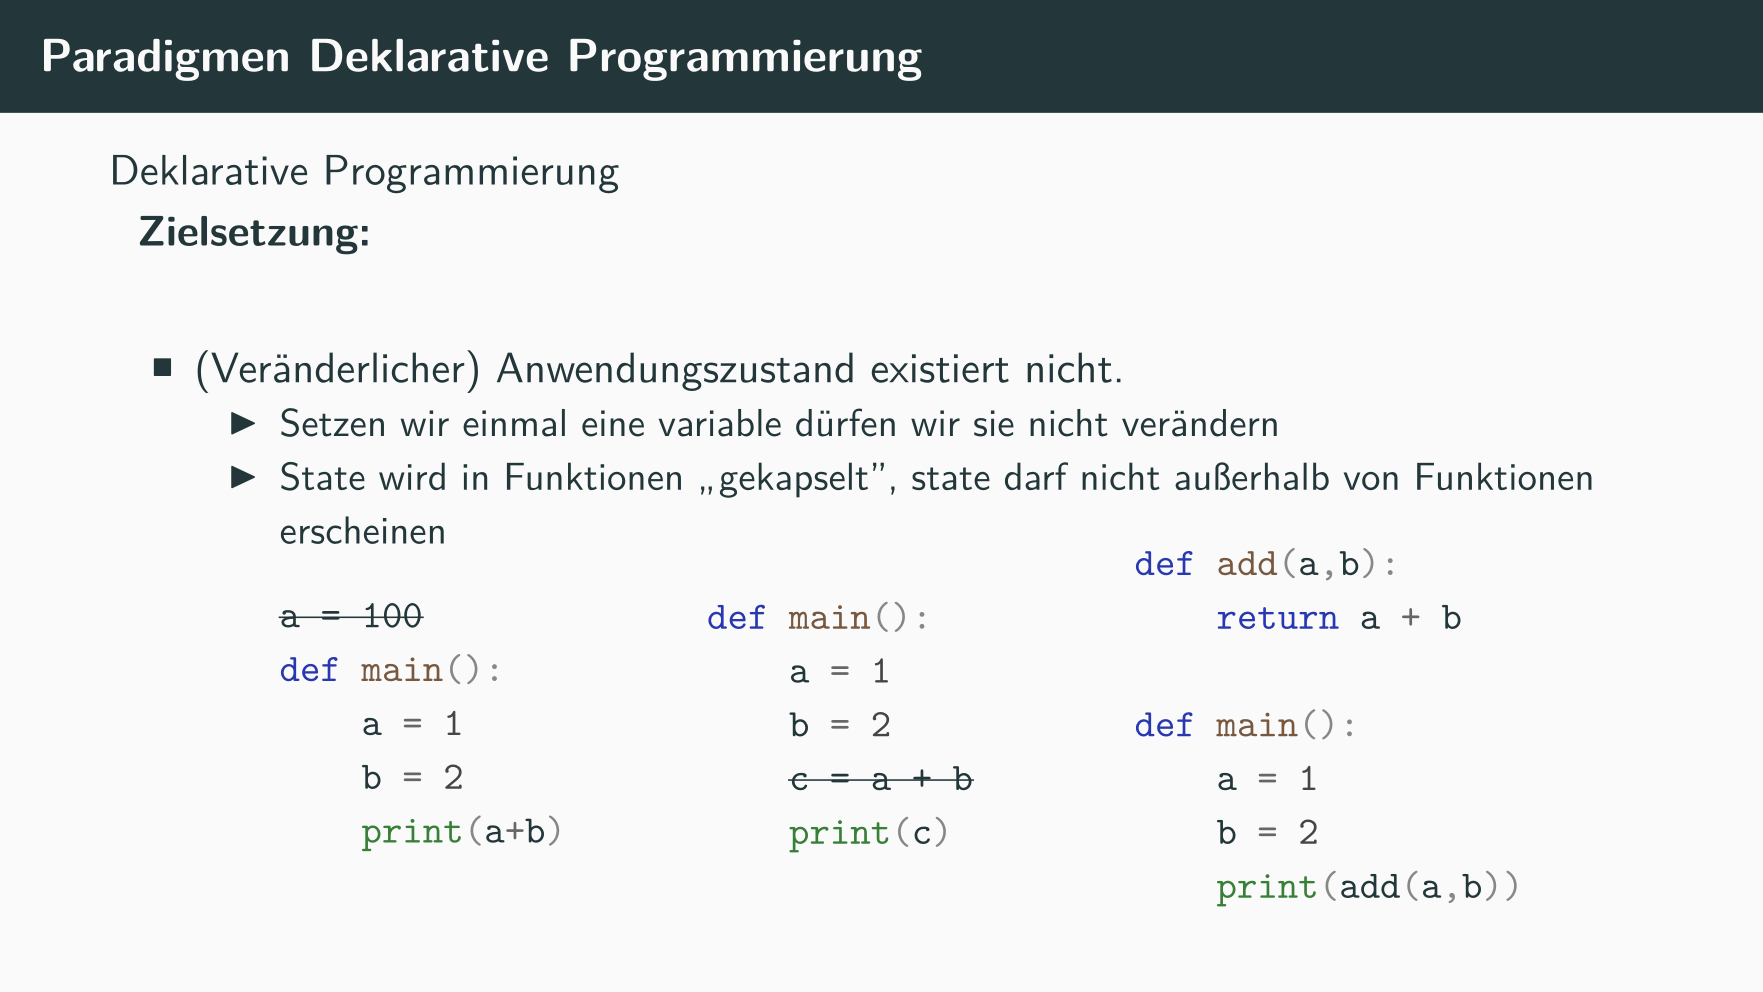
\includegraphics[width=.8\linewidth]{assets/2025-11-19-15-57-07.png}}
Gaaaaaaaanz viele code beispiele folgen!
}


\begin{frame} [fragile]
    \frametitle{Paradigmen -- Deklarative Programmierung}
    {\large Ein naiver Versuch:}\\\vspace{2em}

    \begin{minipage} {.4\linewidth}
    \begin{minted} {python}
def main():
    werte = [1,2,3,4,5]
    summe = 0
    for wert in werte:
        summe = summe + wert

main()
    \end{minted}
    \end{minipage}
\end{frame}
\begin{frame} [fragile]
    \frametitle{Paradigmen -- Deklarative Programmierung}
    {\large Ein naiver Versuch:}\\\vspace{2em}

    \begin{minipage} {.4\linewidth}
    \begin{minted} {python}
def main():
    werte = [1,2,3,4,5]
    summe = 0
    for wert in werte:
        summe = summe + wert

main()
    \end{minted}
    \end{minipage}
    \hspace{.15\linewidth}
    \begin{minipage} {.4\linewidth}
        \begin{minted}[escapeinside=||] {python}
def main():
    werte = [1,2,3,4,5]
    summe = 0
    |\sout{for wert in werte:}|
        |\sout{\texttt{summe = summe + wert}}|

main()
    \end{minted}
    \end{minipage}
\end{frame}

\begin{frame} [fragile]
    \frametitle{Paradigmen -- Deklarative Programmierung}
    \vspace{.3em}
    {\large Neue Spielregel:}\\
    % \vspace{.3em}

    \begin{minipage} {.55\linewidth}
        \begin{minted}[escapeinside=||] {python}
def f(a):
    return a() + 2

def a():
    return 1

def main():
    funktion = a
    print(funktion())  # schreibt 1
    print(f(funktion)) # schreibt 3
    print(f(a))        # schreibt 3

    \end{minted}
    \end{minipage}
    
\end{frame}

\begin{frame} [fragile]
    \frametitle{Paradigmen -- Deklarative Programmierung}
    \vspace{.3em}
    {\large Neue Spielregel:}\\
    % \vspace{.3em}

    \begin{minipage} {.55\linewidth}
        \begin{minted}[escapeinside=||] {python}
def f(a):
    return a() + 2

def a():
    return 1

def main():
    funktion = a
    print(funktion())  # schreibt 1
    print(f(funktion)) # schreibt 3
    print(f(a))        # schreibt 3

    \end{minted}
    \end{minipage}
    \begin{minipage} {.4\linewidth}
        {\large\bf Ein Designpattern!}~\\\vspace{.6em}

        Das ""Callback-Pattern"":\\

        Eine \textrm{Funktion} kann als \textrm{Parameter} einer anderen \textrm{Funktion} verwendet werden.

        \vspace{.9em}
        \vfill
    \end{minipage}
    \vfill
    
\end{frame}

\begin{frame}[fragile]
    \frametitle{Paradigmen -- Deklarative Programmierung}
    \vfill
        \begin{minipage} {.4\linewidth}
        \begin{minted}[escapeinside=||] {python}
def foreach_once(fn, liste, index):
    fn(liste[index])
    if index < (len(liste)-1):
        foreach_once(fn, liste, index + 1)

def foreach(fn, liste):
    foreach_once(fn, liste, 0)

def do_for_all(element):
    print(element)

def main():
    liste = [1,2,3,4,5]
    foreach(do_for_all, liste)
    \end{minted}
    \end{minipage}
\end{frame}

\begin{frame}[fragile]
    \frametitle{Paradigmen -- Deklarative Programmierung}
    \vfill\vspace{.3em}
        \begin{minipage} {.4\linewidth}
            \begin{minted}[escapeinside=||, fontsize=\fontsize{8pt}{9pt}] {python}
def reduce_once(fn, akk, liste, index):
    if index < len(liste):
        newakk = fn(akk, liste[index])
        res = reduce_once(fn, newakk, liste, index + 1)
        return res
    else:
        return akk

# Reduziert die Liste liste mithilfe der Funktion fn zu einem einzelnen Wert
def reduce(fn, akk, liste):
    return reduce_once(fn, akk, liste, 0)

def do_for_all(akk, wert):
    return akk + wert

def main():
    liste = [1,2,3,4,5]
    akk = 0
    summe = reduce(do_for_all, akk, liste)
    print(summe)
    \end{minted}
    \end{minipage}
    \vspace{.3em}
\end{frame}

\begin{frame}[fragile]
    \frametitle{Paradigmen -- Deklarative Programmierung}
    {\large Klingt unnötig kompliziert?}
        \begin{outline}
            \1 Ein einfacheres Beispiel:
            \2[]\begin{minted} {python}
werte = [1,2,3,4,5]
summe = sum(werte)
print(summe)
            \end{minted}
            \vfill
        \1 Ist äquivalent zu:
        \2[]\begin{minted}[fontsize=\fontsize{9}{11}] {python}
def do_for_all(akk, wert):
    return akk + wert

werte = [1,2,3,4,5]
akk = 0
summe = reduce(do_for_all, akk, werte)
print(summe)
            \end{minted}
        \end{outline}
\end{frame}

\begin{frame}[fragile]
    \frametitle{Paradigmen -- Deklarative Programmierung}
    
    \begin{outline}
        \0 {\large Ein letztes:}
        \1[] Eine Funktion, die mehrere Parameter nimmt kann wie folgt in eine Serie von Funktionen aufgebrochen werden:
        \1[] \begin{minted}[fontsize=\fontsize{9}{11}] {python}
def add(a, b):
    return a + b

def add_curried(a):
    def add_b(b):
        return a + b
    return add_b

add5 = add_curried(5) # Erzeugt eine Funktion, die 5 + b rechnet
print(add5(3))        # Ausgabe: 3 + 5 = 8

        \end{minted}
        \1[] Diese Praxis heißt \textbf{Currying}.
    \end{outline}
\end{frame}
